% % % % % % % % % % % % % % % % % % % % % % % % % % % % % % % % % % % % % % % % % % % %
%                                                                                     %
% Short Sectioned Assignment LaTeX Template Version 1.0 (5/5/12)                      %
% This template has been downloaded from: http://www.LaTeXTemplates.com               %
%                                                                                     %
% Original author:  Frits Wenneker (http://www.howtotex.com)                          %
%                                                                                     %
% Modified by: Fco Javier Sueza Rodríguez (fcosueza@disroot.org)                      %
%                                                                                     %
% Changes:                                                                            %
%	    - Custom Chapters, Sections and Subsections (titlesec package)                %
%           - Document type scrbook (oneside)                                         %
%           - Use babel-lang-spanish package and marvosym                             %
%           - Use hyperref, enumitem, tcolorbox and glossaries packages               %
%           - Use Time New Roman (mathptmx), Helvetic and Courier fonts               %
%                                                                                     %
% License: CC BY-NC-SA 3.0 (http://creativecommons.org/licenses/by-nc-sa/3.0/)        %
%                                                                                     %
% % % % % % % % % % % % % % % % % % % % % % % % % % % % % % % % % % % % % % % % % % % %

%-----------------------------------------------%
%	              Packages                  %
%-----------------------------------------------%

\documentclass[paper=a4, fontsize=11pt, oneside]{scrbook}

% ---- Text Input/Output ----- %

\usepackage[T1]{fontenc}
\usepackage[utf8]{inputenc}
\usepackage{mathptmx}
\usepackage[scaled=.92]{helvet}
\usepackage{courier}
\usepackage[indent=12pt]{parskip}

\usepackage{geometry}
\geometry{verbose,tmargin=3cm,bmargin=3cm,lmargin=2.6cm,rmargin=2.6cm}

% ---- Language ----- %

\usepackage[spanish]{babel}
\usepackage{marvosym}

% ---- Another packages ---- %

\usepackage{amsmath,amsfonts,amsthm}
\usepackage{graphics,graphicx}
\usepackage{titlesec}
\usepackage{fancyhdr}
\usepackage{tcolorbox}
\usepackage{hyperref}
\usepackage{enumitem}
\usepackage[automake]{glossaries}

%--------------------------------------------------------------------%
%                      Customizing Document                          %
%--------------------------------------------------------------------%


% ----------- Custom Chapters, Sections and Subsections -------------- %

\titleformat{\chapter}[display]
			{\bfseries\Huge}
			{Tema \ \thechapter} {0.5ex}
			{\vspace{1ex}\centering}

\titleformat{\section}[hang]
			{\bfseries\Large}
			{\thesection}{0.5em}{}

\titleformat{\subsection}[hang]
			{\bfseries\large}
			{\thesubsection}{0.5em}{}

\titleformat{\subsubsection}[hang]
			{\bfseries\large}
			{\thesubsubsection}{0.5em}{}

\hypersetup{
    colorlinks=true,
    linkcolor=black,
    urlcolor=magenta
}

% ------------------- Custom heaaders and footers ------------------- %

\pagestyle{fancyplain}

\fancyhead[]{}
\fancyfoot[L]{}
\fancyfoot[C]{}
\fancyfoot[R]{\thepage}

\renewcommand{\headrulewidth}{0pt} % Remove header underlines
\renewcommand{\footrulewidth}{0pt} % Remove footer underlines

\setlength{\headheight}{13.6pt} % Customize the height of the header

% --------- Numbering equations, figures and tables ----------------- %

\numberwithin{equation}{section} % Number equations within sections
\numberwithin{figure}{section} % Number figures within sections
\numberwithin{table}{section} % Number tables within sections

% ------------------------ New Commands ----------------------------- %

\newcommand{\horrule}[1]{\rule{\linewidth}{#1}} % Create horizontal rule command


%----------------------------------------------------------------------------------------
%	TÍTULO Y DATOS DEL ALUMNO
%----------------------------------------------------------------------------------------

\title{
\normalfont \normalsize
\textsc{{\bfseries Curso 2023-2024} \\ Ciclo Superior de Desarrollo de Aplicaciones Web \\ IES Aguadulce} \\ [25pt]
\horrule{0.5pt} \\[0.4cm]
\huge Empresa e Iniciativa Emprendedora \\
\horrule{0.5pt} \\[0.4cm]
}

\author{Francisco Javier Sueza Rodríguez}
\date{\normalsize\today}

%----------------------------------------------------------------------------------------
%                                     DOCUMENTO
%----------------------------------------------------------------------------------------
\makeglossaries
\loadglsentries{glossary.tex}

\begin{document}

\maketitle

\newpage

\tableofcontents

\listoffigures

%\listoftables

\newpage

\chapter{La Empresa y su Clasificación}
En este primer tema, vamos en que consiste una empresa, dando su definición y explicando los diferentes elementos que la componen, tanto humanos como materiales, así como de su organización. También hablaremos sobre la función y finalidad que tiene una empresa, hablaremos de la ética empresarial y daremos una clasificación de la empresa según diferentes características.

\section{Empresa e Iniciativa Emprendedora}
En este módulo pretendemos \textbf{conocer más sobre la empresa}. A diferencia de la asignatura de \textbf{Formación y Orientación Laboral}, donde se adopta el punto de vista del trabajador, nosotros adoptaremos el punto de vista del empresario o empresaria, porque tu también puede llegar a serlo, y porque, aunque trabajes por cuenta ajena, también necesita saber como colaborar para que tu empresa pueda mejorar.

El concepto de empresa puede ser definido desde ópticas muy diferentes: llamamos empresa al lugar de trabajo, a una acción o tarea que entrañe dificultades y cuya ejecución requiere decisión y esfuerzo, a la unidad organizada que desarrolla una actividad económica, etc. Partiendo de esta última perspectiva, vamos a definir la empresa.

Una \textbf{empresa} es un conjunto de \textbf{elementos humanos y materiales organizados} dedicado a la \textbf{producción de bienes} y/o la prestación de \textbf{servicios} dirigidos a satisfacer necesidades humanas, con ánimo de obtener un \textbf{beneficio}.

\section{Elementos de una Empresa}
Podemos establecer, de una forma muy simplificada, que los elementos de una empresa son los que podemos ver en la siguiente figura.

\begin{figure}[H]
    \centering
    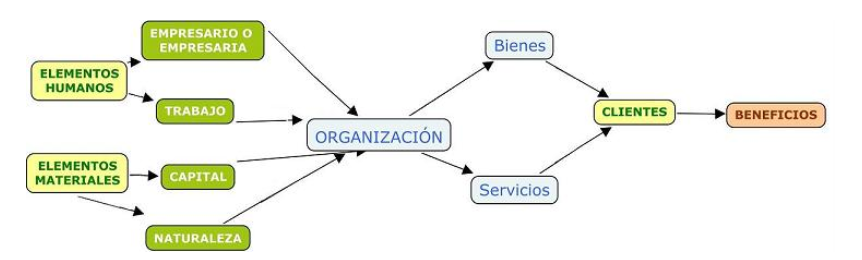
\includegraphics[scale=0.50]{elementos-empresa.png}
    \caption{Elementos de una empresa}
\end{figure}

En los siguiente puntos, vamos a analizaremos algunos de estos elementos.

\subsection{Los Elementos Humanos}
En primer lugar, vamos a ver cuales son los elementos humanos que componen una empresa, pudiendo diferenciar principalmente entre los siguientes dos elementos:

\begin{itemize}
    \item \textbf{Empresaria o Empresario}: es la persona o grupo de éstas que aporta \textbf{el capital} para el desarrollo de la actividad empresarial y asume \textbf{los riesgos} que de ella se deriven con la intención de obtener un beneficio económico.

    \item \textbf{Trabajadores y Trabajadoras}: tradicionalmente llamados recursos humanos, a nosotros nos gusta más llamarlo equipo de trabajo. Se trata de las personas que dedican su tiempo y esfuerzo a las actividades productivas a cambio de una remuneración, de una \textbf{salario}. Comprende cualquier tipo de \textbf{actividad humana}, ya sea física o intelectual y muy diferentes niveles de cualificación: trabajadores no cualificados, técnicos, mandos intermedios, directivos, etc.
\end{itemize}

\subsection{Los Elementos Materiales}
Los principales elementos materiales de una empresa son los recursos naturales y el capital, que describimos a continuación.

\begin{itemize}
    \item \textbf{Recursos Naturales}: son recursos naturales elementos como el agua, energía, arboles, animales, viento, etc...

    \item \textbf{Capital}: se puede considerar capital  al dinero, acciones, patentes, marcas, edificios, instalaciones, maquinarias, productos semielaborados y los demás medios materiales que intervienen en el proceso de producción. Pueden ser duraderos o no duraderos en el tiempo.
\end{itemize}

\subsection{La Organización}
Para que una empresa funcione debe estar organizada. La \textbf{organización} consiste en la coordinación de los elementos humanos y materiales de que se disponen, a fin de obtener mejor rendimiento  de los mismos.

Este \textbf{rendimiento óptimo} de los recursos disponibles procura una cantidad  y calidad deseadas, de un producto o servicio, en un tiempo determinado con un mínimo de coste, de tal forma que satisfaga las necesidades del consumidor. Si la empresa esta bien organizada, decimos que es \textbf{productiva}.

Para entender lo que es el \textbf{rendimiento óptimo} vamos a ver el siguiente ejemplo:

Un restaurante va cada vez mejor y tiene muchos clientes fijos que van a comer allí todos los días. Se ha hecho un cálculo atendiendo al método y tiempos de trabajo de la empresa y se ha determinado que se puede atender al día satisfactoriamente a 40 clientes, ¿que ocurriría si intentarán atender a 50 personas o a todas las que acudan al restaurante? ¿Cómo se sentirían los trabajadores? ¿Y los clientes? ¿Es más conveniente decirles que vuelvan otro día? A la larga, intentar maximizar los rendimientos de la empresa puede tener consecuencias negativas: empeora el clima laboral, menor calidad del servicio, problemas de espacio, incumplimiento de tiempos, clientes insatisfechos y cansados de esperar, etc...

\section{Funciones de la Empresa}
Para cumplir con sus objetivos, las empresas desarrollan un serie de \textbf{actividades} diferentes que se agrupan por divisiones, áreas, departamentos,... las denominaremos, \textbf{funciones de la empresa}.

Podemos clasificar las funciones de una empresa en:

\begin{itemize}
    \item \textbf{Función comercial}: son las actividades relacionadas con la compraventa, como investigar el mercado, hacer acopio de los materiales necesarios, obtención del producto, ponerle precio, etc...
    \item \textbf{Función de producción, de operaciones o técnica}: son las actividades relativas al diseño del producto, el proceso de producción y transformación de las materias primas, gestión del almacén, etc..
    \item \textbf{Función financiera y contable}: se encarga de la obtención del capital, control de los ingresos y gatos, documentación, etc...
    \item \textbf{Función social}: tiene que ver con el equipo humano que compone la empresa, determinar que tipo de personas deben ser, los tipos de contratos que se van a realizar, etc..
    \item \textbf{Función directiva}: es la función encargada de coordinar todas las funciones anteriores, planificando y organizando todas las funciones para que la empresa pueda llegar a sus objetivos.
\end{itemize}

Para que todas estas funciones trabajen adecuadamente hay que tener en cuenta lo siguiente:

\begin{itemize}
    \item \textbf{Dependencia}: la efectividad de una empresa no depende de un área funcional específica, sino de la coordinación de todas ellas.

    \item \textbf{Graduación de la importancia}: las funciones no revisten la misma importancia en todas las empresas. A veces algunas dominan sobre el resto, incluso puede suceder que haya alguna que carezca de relevancia. Por ejemplo, en una tienda de ropa, la función más relevante es la comercial, mientras que realmente no hay una función de producción.
\end{itemize}

La \textbf{importancia de una función} va a depender de la actividad que desarrolle la empresa, el tamaño, el número de personas implicadas, etc.

Por ejemplo, en una empresa individual todas las funciones son realizadas por al misma persona, mientras que en una multinacional, con cientos de personas trabajando, las funciones se multiplican y aparecen algunas nuevas como la Investigación, Desarrollo e Innovación (I+D+I), control de calidad, seguridad, etc.

Como veremos en temas sucesivos, las funciones de la empresa se corresponden con los apartados del \textbf{plan de negocio}, pero no adelantemos acontecimientos...

\section{Finalidad de una Empresa: La Satisfacción de Necesidades}
Tradicionalmente se considera que la finalidad de una empresa es la obtención de beneficios, pero el beneficio no debe ser la finalidad principal del comportamiento o las decisiones de la empresa actual, sino, la razón de su existencia.

Los \textbf{beneficios son el resultado} indispensable sin el cual los negocios no pueden sobrevivir, pero una empres que considere los beneficios como su meta principal puede ser que no llegue a conseguir sus objetivos. Vamos a intentar explicarlo mejor, la \textbf{finalidad objetiva} que debe tener en cuenta una empresa moderna es la \textbf{creación de clientes}, clientes satisfechos y fieles a los productos o servicios objeto de la actividad de la empresa. La \textbf{satisfacción} de las \textbf{necesidades de los consumidores} es la base de supervivencia de la empresa y de su crecimiento futuro.

Pero los clientes y consumidores somos cada vez más exigentes y el mundo empresarial es muy competitivo. Las empresas deben conocer estas exigencias y adaptarse a los cambios, conocer su entorno, comportarse de forma ética y asumir su responsabilidad social. Es lo que vamos a ver en los siguiente apartados.

\section{La Cultura de Empresa y la Imagen Corporativa}
La \textbf{empresa es un sistema}, una entidad formada por una serie de elementos, con unas determinadas funciones, que se relacionan con el exterior. Pero, ¿ que b\textbf{valores y principios} sustentan las elecciones de la empresa? ¿Cómo quiere ser?

Toda empresa tiene unos \textbf{pilares básicos} a la hora de \textbf{dirigir sus actuaciones}, un conjunto de creencias, valores, principios... que rigen su funcionamiento, que son asumidos y compartidos por las personas y los grupos que la integran y que se manifiestan en la forma en la que interaccionan con otros y ellos con el entorno, es la \textbf{cultura empresarial}.

La cultura de una organización la hace \textbf{diferente} de otros y condiciona los \textbf{objetivos} que se fijan y las \textbf{estrategias} que se siguen para lograrlos. Para que la cultura de la empresa sea aceptada y asumida por el equipo humano que la integra es necesario que las personas que dirigen la organización ejerzan un \textbf{liderazgo} eficaz que garantice la interpretación correcta de los elementos culturales.

Algunas empresas orientan su cultura \textbf{al poder}, otras se preocupan de la \textbf{función}, otras se orientan a la \textbf{consecución de objetivos} y resultados fomentando, por ejemplo, la planificación y el trabajo en equipo.

En los últimos tiempos se esta incrementando el número de empresas que centran su atención en \textbf{las personas}, en el \textbf{equipo humano}, tratando de satisfaces sus necesidades sociales y potenciando su desarrollo personal y profesional. Su estructura, con \textbf{pocos niveles de autoridad}, fomenta la participación y el consenso de decisiones. El bienestar de los empleados, la realización laboral y la conciliación de la vida laboral y personal podrían ser algunos de sus valores.

La \textbf{imagen corporativa} de una empresa es la imagen que la empresa proyecta al exterior, lo que la gente piensa y siente acerca de lo que la empresa es y como actúa. El logotipo, la decoración, los uniformes de la empresa, los colores distintivos, el eslogan, la música... incluso el olor, son símbolos que trasmiten una imagen, una personalidad de la empresa y que influyen en su éxito o fracaso. Es importante, que la imagen que se perciba de la empresa este acorde con la imagen que ésta quiere transmitir.

\section{La Ética Empresarial}
\textbf{La ética} es la parte de la Filosofía que estudia la moral y determina que es lo bueno (o lo malo), lo correcto (o lo incorrecto), lo permitido (o no permitido) y como se debe actuar. La empresa actúa y sus actuaciones tiene unas repercusiones positivas o negativas sobre las personas que la integran y su entorno.Estos principio se recogen en un \textbf{código de conducta} que se convierte en la expresión escrita de la cultura de la empresa.

El \textbf{comportamiento no ético} en la empresa tiene muchas consecuencias negativas, entre ellas:

\begin{itemize}
    \item Desprestigio y mala imagen.
    \item Pérdida de clientes.
    \item Trabajadores descontentos, desmotivados, improductivos o que dejan la empresa.
    \item Proveedores que no quieren establecer relaciones comerciales.
    \item Bancos que no aprueban créditos.
    \item Perdida de relaciones con la Administración, perdida de posibles subvenciones o ayudas.
    \item Sanciones jurídicas, cuando además los actos no éticos incumplen las normas jurídicas.
\end{itemize}

Como vemos, las consecuencias de llevar a cabo acciones poco éticas pueden ser muchas y muy perjudiciales para una empresa.

\section{La Responsabilidad Social de las Empresas}
La \textbf{responsabilidad social} (RSE) supone que la empresa toma en consideración las repercusiones que sus actividades tienen en el entorno y en la sociedad y asume voluntariosamente \textbf{compromisos} que van más allá de las obligaciones legales, que debe cumplir en cualquier caso, y por los que pretende contribuir al desarrollo sostenible y por los que intenta:

\begin{itemize}
    \item Elevar los niveles de desarrollo social.
    \item Proteger el medio ambiente.
    \item Respetar los derechos humanos.
    \item Adoptar un modo de dirección abierto que reconcilie los diferentes agentes sociales.
\end{itemize}

En el años 2000, se desarrollo el \href{https://www.pactomundial.org/noticia/10-principios-17-ods/}{Pacto Mundial} de las Naciones Unidas, que es un llamado a las empresas del mundo para que voluntariamente alineen las estrategias. En 2015 se firmó la Agenda 2030 que está en línea con los 10 principios del Pacto Mundial.

Las empresas españolas tiene cada vez más en cuenta los ODS (Objetivos de Desarrollo Sostenible) a la hora de definir y redefinir su Responsabilidad Social Corportativa (RSC), sus objetivos y sus metas. En términos generales, las empresas nacionales coinciden en destacar la priorización de tres de los ODS: \textbf{ODS 8} ``Trabajo decente y crecimiento económico'', \textbf{ODS 5} ``Igualdad de género'' y \textbf{ODS 3} ``Salud y bienestar'', destacando dos áreas críticas en las empresas que requieren medidas inmediatas  a nivel internacional: \textbf{la lucha contra el cambio climático} y \textbf{la igualdad de género}.

Pasa saber más sobre los ODS puede consultar \href{https://www.pactomundial.org/noticia/10-principios-17-ods/}{la página de la ONU} referente al tema, donde los explica todos con más detalles.

Para \textbf{gestionar la responsabilidad social} se podrían llevar a cabo los siguientes pasos:

\begin{itemize}
    \item \textbf{Analizas y diagnosticar} la situación de la empresa.
    \item Establecer un \textbf{código propio de normas} en el que se recojan las medidas que se pretenden adoptar para que la cultura de empresa y sus acciones sean éticas y socialmente responsables.
    \item Poner en \textbf{práctica} estas medidas.
    \item \textbf{Evaluar} los resultados de su aplicación.
    \item Adoptar las \textbf{medidas correctoras} oportunas para mejorarlo.
\end{itemize}

El instrumento de gestión que permite registrar, evaluar, organizar y planificar la gestión social de una empresa en términos cualitativos y cuantitativos se denomina \textbf{balance social} o \textbf{memoria sostenible}.

\section{Estrategias para Ser Socialmente Responsable}
La responsabilidad social debe manifestarse en las relaciones de la empresa con los grupos de interés. Se denomina \textbf{grupos de interés} o \textbf{stakeholders} a las personas o grupos de personas que afectan o se ven afectados por la actividades, productos o servicios de una empresa u organización.

A continuación vamos a ver algunos ejemplos de \textbf{actuaciones} o \textbf{medidas} que implican asumir la responsabilidad social y los grupos a los que afecta.

\begin{itemize}
    \item \textbf{Con el grupo humano que compone la empresa}:
    \begin{itemize}
        \item Hacer la no discriminación social este presente en el proceso de selección de personal, facilitando de inserción laboral de discapacitados, mujeres, parados de larga duración, etc...
        \item Establecer condiciones de trabajo seguras, saludables y justas.
        \item Potencias las capacidades y competencias del equipo y proporcionarles los recursos que requieren para realizar sus tareas.
        \item Fomentar la participación en las decisiones y la responsabilidad.
        \item Permitir la participación en los beneficios.
        \item Llevar una gestión ética, clara y transparente.
    \end{itemize}

    \item \textbf{Con los consumidores y clientes}:
    \begin{itemize}
        \item Establecer canales de comunicación fluida.
        \item Averiguar el grado de satisfacción y fidelidad de los clientes.
        \item Tener en cuenta posibles limitaciones personales de los clientes, como discapacidades, mayores, menores,...
        \item Aplicar principios éticos a la publicidad y promociones.
        \item Responder de la calidad del producto o servicio.
        \item Certificar que el negocio es socialmente responsable y posee los criterios exigidos de calidad.
    \end{itemize}

    \item \textbf{Con los proveedores}:
    \begin{itemize}
        \item Actuar con ética en las relaciones que se mantienen con éstos.
        \item Cumplir los plazos de entrega y pagos.
        \item Medir el grado de satisfacción que tienen respecto al negocio.
        \item Al elegirlos, fijarse si son socialmente responsables.
    \end{itemize}

    \item \textbf{Con los competidores}
    \begin{itemize}
        \item Tratar de llegar a acuerdos con ellos en materia de RSE.
        \item Evitar la competencia desleal, la agresión o el juego sucio.
        \item Potenciar la cooperación.
        \item Participar en eventos que traten de fomentar la RSC y compartir con las otras empresas las buenas prácticas.
    \end{itemize}

    \item \textbf{Con los inversores}:
    \begin{itemize}
        \item Proporcionar información transparente sobre la gestión económica de la empresa.
        \item Elaborar una memoria de sostenibilidad y utilizar la web para darla a conocer.
    \end{itemize}

    \item \textbf{Con el medioambiente}:
    \begin{itemize}
        \item Además de cumplir con las leyes sobre medioambiente, acudir a ONGs y asociaciones para asesorarse.
        \item Buscar alianzas ecológicas con posibles proveedores.
        \item Analizar el consumo de recursos de la empresa y reducirlo si es posible.
        \item Utilizar material reciclado y comunicarlo.
        \item Suministrar servicios y productos respetuosos con el medioambiente.
    \end{itemize}

    \item \textbf{Con la comunidad}:
    \begin{itemize}
        \item Realizar donaciones o patrocinar iniciativas sociales, culturales o deportivas.
        \item Cooperar con ONGs e instituciones de cooperación y desarrollo.
        \item Las acciones se pueden dar a conocer a través de guías, etiquetado de productos, embalajes, etc...
    \end{itemize}

    \item \textbf{Con la administración}:
    \begin{itemize}
        \item Demostrar un comportamiento ético con la administración sin eludir las responsabilidades legales, como cumplir con los tramites, pago de impuestos, etc...
        \item Colaborar en proyectos de interés general.
    \end{itemize}
\end{itemize}

A pesar de esto, las \textbf{acciones de los gobiernos} no están siendo suficientes para corregir los desajustes sociales, económicos y medioambientales, aunque cada vez más \textbf{consumidores} no solo quieren productos buenos y seguros, sino también que se \textbf{produzcan y procesen} de \textbf{manera responsable}.

En este aspecto, existen \textbf{etiquetas sociales} y \textbf{ecológicas} por parte de los distintos fabricantes, como los sellos AENOR medioambiente, FSC, certificado FER, Comercio Justo, certificado Welfare, etc...

\section{Tipos de Empresas}
Las empresas se pueden clasificar atendiendo a diferentes criterios. En este apartado, analizaremos las clasificaciones que puedan sernos útiles con los siguientes objetivos:

\begin{itemize}
    \item Tener una visión global del tejido empresarial nacional e internacional.
    \item Encuadrar una empresa concreta en cada una de las clasificaciones más usuales.
    \item Comprender algunos conceptos que se utilizan con mucha frecuencia y cuyo significado puede que no tengamos claro, como pueden ser: PYMES, empresas de servicios, franquicia, monopolio, holding, etc...
\end{itemize}

Para ello, atenderemos a los \textbf{siguiente criterios} para realizar la clasificación de las empresas:

\begin{itemize}
    \item La actividad económica.
    \item El sector económico.
    \item La dimensión.
    \item El ámbito geográfico.
    \item La titularidad del negocio.
\end{itemize}

Dejaremos la clasificación jurídica de las empresas para temas posteriores debido a su importancia y complejidad.

\subsection{Clasificación de Empresas Según su Actividad Económica}
En este apartado vamos a ver la clasificación de las empresas atendiendo al criterio de la actividad económica que realizan, para ello, vamos a usar un esquema que puedes ver en la siguiente figura.

\begin{figure}[H]
    \centering
    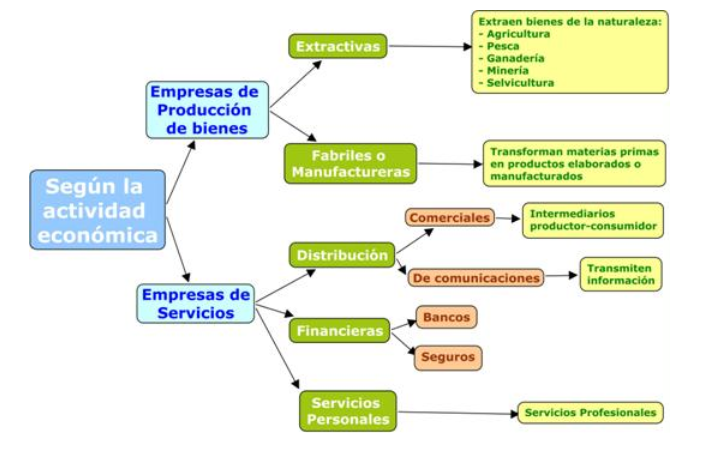
\includegraphics[scale=0.60]{empresas-actividad-economica.png}
    \caption{Clasificación de empresa por actividad económica}
\end{figure}

Si quieres saber más, puedes consultar la página web del INE, en concreto, nosotros te recomendamos los datos sobre empresas del \href{https://www.ine.es/prensa/dirce_2019.pdf}{DIRCE}.

\subsection{Clasificación de Empresas Según Sector Económico}
En este apartado vamos a presentar una clasificación de empresas que atiende al sector económico en las que estas desarrollan su actividad. Los sectores económicos que podemos encontrar los vemos en el siguiente esquema.

\begin{figure}[H]
    \centering
    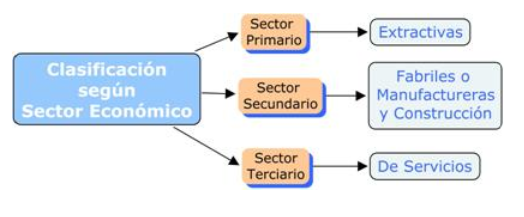
\includegraphics[scale=0.50]{sectores-economicos.png}
    \caption{Sectores económicos}
\end{figure}

Desde hace poco tiempo, debido a su creciente importancia y expansión, algunos autores han añadido un nuevo sector: \textbf{el ``cuaternario''}. Se incluyen en ellas empresas relacionadas con las nuevas tecnologías, la tecnologías de las información, la investigación y el desarrollo y la innovación.

Las empresas normalmente centran su actividad en un sector concreto pero puede haber grandes empresas o grupos de empresas que \textbf{desarrollen su actividad} en \textbf{más de un sector} o incluso en tres sectores. Imagina por ejemplo una multinacional de restaurantes de comida rápida que tiene sus propias ganaderías, fábricas en las que elabora sus productos y cientos de restaurantes repartidos por todo el mundo.

Para determinar el \textbf{grado de desarrollo de un país} se puede analizar el porcentaje que representa cada uno de los sectores sobre el Producto Interior Bruto. Con carácter general, en los países que predomina el sector primario suelen ser países subdesarrollados, mientras que si predomina el sector servicios suelen ser países con un alto nivel de desarrollo.

\subsection{Clasificación Según su Dimensión}
Las empresas se clasifican en  \textbf{pequeña}, \textbf{mediana} y \textbf{grande} según su dimensión, pero hay que tener en cuenta varios criterios para realizar esta clasificación.

Un primer criterio puede ser el número de trabajadores que tiene. Puede suceder que una empresa tenga mucho capital, muchos beneficios, proyección,... pero una plantilla reducida porque todo su proceso de producción este mecanizado. Esto ocurre, por ejemplo, en la grandes compañías cementeras. O al contrario, podría haber una empresa con muchos trabajadores en su proceso de producción pero que no sean demasiado grandes.

Por esto, para clasificar a una empresa según su dimensión no podemos tener solo en cuenta el número de trabajadores, sino que además, habrá que tener en cuenta, entre otros, lo siguiente:

\begin{itemize}
    \item El volumen de ventas
    \item El capital social
    \item Los beneficios
    \item El ámbito geográfico
    \item El número de sucursales..
\end{itemize}

En la siguiente tabla podemos ver la clasificación atendiendo a algunos de estos criterios. Para que una empresa se considere dentro de una clasificación, además del número de trabajadores, debe cumplir alguno de los otros dos requisitos.

\begin{figure}[H]
    \centering
    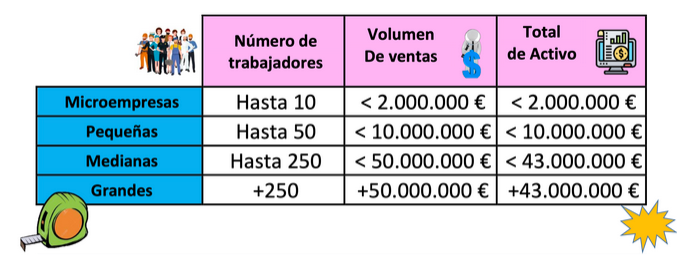
\includegraphics[scale=0.50]{empresas-dimension.png}
    \caption{Clasificación de empresas según su dimensión}
\end{figure}

\subsection{Las PYMES}
Dentro de la clasificación por dimensión que hemos realizado de las empresas merecen mención aparte las \textbf{PYMES} (Pequeñas Y Medianas EmpresaS). Esta empresas suelen encontrarse con \textbf{problemas específicos} como pueden ser los siguientes:

\begin{itemize}
    \item Carencia de tecnología o capacidad de investigación.
    \item Dificultad en el acceso a al información.
    \item Competencia con grandes empresas.
    \item Menor fuerza para presionar a los proveedores y reducir costes.
    \item Financiación casi exclusiva a través de los bancos, lo que hace que los créditos sean más caros.
\end{itemize}

A pesar de esto, las \textbf{PYMES} también tiene sus \textbf{ventajas}, como pueden ser:

\begin{itemize}
    \item Posibilidad de dar un trato más personal al cliente.
    \item Poder cubrir los huecos que las grandes empresas dejan con clientes insatisfechos.
    \item Atraer a personas con talento a las que no les gusta trabajar en grandes empresas.
    \item Mayor flexibilidad para adaptarse a los cambios..
\end{itemize}

Cabe también hablar en este apartado de las \textbf{Startups}. Una \textbf{Startup} es una empresa de nueva creación o edad temprana que presenta grandes posibilidades de crecimientoy comercializa productos y servicios a través del uso de las nuevas tecnologías.

Es relevante \textbf{saber distinguir} entre una \textbf{PYME} y una \textbf{Startup}. Las pymes convencionales salen al mercado después de haber invertido una cantidad de dinero y deben esperar un tiempo hasta empezar a ver beneficios. Las startups, en cambio, salen rápidamente al mercado para lograr el crecimiento y la financiación necesarios a través de las transformación digital.

Las principales \textbf{características} de una starup son las siguientes:

\begin{itemize}
    \item \textbf{Jóvenes}: compañías familiarizadas con una ambiente joven, moderno, tecnológico, que tras nacer, intentan conseguir financiación.
    \item \textbf{Escalables}: es principal atributo de la startup es la velocidad y la capacidad con la que pueden crecer y generar ingresos de una forma rápida.
    \item \textbf{Tecnológicas}: son negocios que se basan en ideas innovadoras para satisfacer una nueva necesidad en el mercado.
    \item \textbf{Pequeños costos}: es punto de partida de las startups es mantener los costos bajos de producción para crecer más rápidamente.
\end{itemize}

\subsection{Clasificación Según el Ámbito Geográfico}
Las empresas también se pueden clasificar según el ámbito geográfico que abarca su actividad. Así podemos encontrar empresas de los siguiente tipos:

\begin{itemize}
    \item \textbf{Locales}: se trata normalmente de pequeñas empresas que desarrollan su actividad en la localidad donde radican o las poblaciones de alrededor.
    \item \textbf{Regionales}: la zona que abarcan es más amplia, comprendiendo varias provincias. Suelen tener una sede central y verifican sus actividades a través de sucursales.
    \item \textbf{Nacionales}: extienden su actividad a toda la geografía nacional.
    \item \textbf{Multinacionales}: son aquellas que ejercen su actividad simultáneamente en varios países. Incluso hay empresas consideradas globales ya que su actividad abarca los 5 continentes.
\end{itemize}

En \textbf{España},  la mayor parte de las empresas son \textbf{locales} o \textbf{regionales}: comercios, empresas de servicios, profesionales, etc. Además, existen \textbf{programas de apoyo} para los emprendedores que dedican \textbf{internacionalizar su negocio}. En Andalucía, el organismo encargado de esta función es Extenda, la Agencia Andaluza de Promoción Exterior.

\subsection{Clasificación Según su Titularidad}
La mayor parte de las empresas españolas son \textbf{privadas}, es decir, que su titular es un particular.

Cuando el capital pertenece al Estado y su titular es una entidad pública estamos antes una \textbf{empresa pública}. Las empresas públicas no solo pretenden la obtención de beneficios, sino que también tienen otros fines como el desarrollo regional, el mantenimiento de puestos de trabajo, la protección de recursos naturales, la actuación sobre sectores estratégicos de la economía, etc... Un ejemplo es la \textbf{Empresa Pública de Emergencias Sanitarias}, cuya web, \href{http://www.epes.es/}{Empresa Pública de Emergencias Sanitarias}.

También existen \textbf{empresas mixtas}, donde una parte del capital pertenece al Estado y otra está en manos privadas.

\section{Las Franquicias}
La \textbf{franquicia} es una fórmula empresarial que nace del acuerdo entre dos personas o empresas: el franquiciador y  el franquiciado.

El \textbf{franquiciador} cede al franquiciado el derecho a fabricar, utilizar o comercializar un producto, un servicio, un nombre o una marca comercial, junto con el conocimiento necesario para realizar el negocio, lo que se conoce como \textbf{Know-how}, a cambio de una contraprestación económica denominada \textbf{canon} o \textbf{royalty}.

El \textbf{franquiciado} realiza la aportación financiera y personal para desarrollar y explotar el negocio comprometiéndose a seguir las normas del franquiciador.

\section{Formas de Concentración Empresaria}
Algunas empresas, a efectos de crecer, alcanzar mayores cuotas de venta o acceder a otros mercados recurren a fusiones, acuerdos o participación en otras empresas. Estamos hablando de lo que se conoce como \textbf{concentración empresarial o industrial}.

Las formas de concentración más importantes que podemos encontrarnos en la actualidad son las siguientes:

\begin{itemize}
    \item \textbf{Cártel}: asociación de empresas del mismos sector que conciertan acuerdos sobre el volumen de producción, precios,... de un mismo producto para incrementar así los beneficios. Están prohibidos por la Unión europea.

    \item \textbf{Trust}: fusión de empresas de un mismo sector que se someten a una misma gestión, perdiendo su independencia y buscando monopolizar o ser más competitivas en algún sector del mercado.

    \item \textbf{Holding Trust}: se trata de una empresa que posee participación en el capital social de otras empresas, controlando su actividad. Están permitidos siempre y cuando no afecten a la libre competencia.

    \item \textbf{Monopolio}: consiste en el control que una sola empresa ejerce sobre un producto o servicio. En Europa no están permitidos.
\end{itemize}

Uno de los casos más conocidos y claros de holdings en nuestro país es el grupo \textbf{Inditex}, que agrupa a conocidas marcas de la industria textil como Zara, Bershka, Pull and Bear o Massimo Dutti.

\section{Las Incubadoras de Empresas}
Algunos organismos públicos apoyan creación de empresas mediante la oferta de \textbf{viveros}, también llamados \textbf{incubadoras}, de empresas.

Se trata de apoyar la creación de negocios durante un determinado tiempo, al inicio de la actividad empresarial, facilitándoles el local y la infraestructura, dándoles apoyo financiero, asesoramiento jurídico, laboral, fiscal, etc...

Instituciones como la Cámara de Comercio tienen viveros de empresas. También puede prestar este tipo de apoyos organismos o instituciones como el Ayuntamiento, la Diputación Provincial, asociaciones de empresarios, universidades, etc...

\section{Empresas de Economía Sumergida}
Las denominadas \textbf{empresas de economía sumergida} realizan actividades económicas eludiendo, total o parcialmente, las normas que regulan la actividad empresarial. Así, estas empresas:

\begin{itemize}
    \item No pagan impuestos.
    \item No cotizan a la Seguridad Social.
    \item Contratan a los trabajadores/as de forma precaria e ilegal.
    \item No cumplen la normativa en seguridad laboral.
    \item Están permanentemente en inestabilidad.
    \item No pueden acceder a créditos o ayudas.
    \item Las personas que las integran no tienen derecho a prestaciones de la Seguridad Social.
    \item Pueden ser multadas por desarrollar actividades fuera de la legalidad.
\end{itemize}

La economía sumergida en España e Italia representa el 20\% del PIB, frente al 13\% de media en la UE. En España es el equivalente a 180.000 millones de euros. El caso extremo de la Comunidad Europea es Grecia, con más del 30\% del PIB.

\section{Material Adicional}
Si te ha interesado el tema y te has quedado con ganas de más, en este último punto vamos a recomendar un conjunto de libros, películas, vídeos y páginas web relacionadas con la empresa y todo lo que hemos visto en este primer tema, especialmente con el emprendimiento.

\begin{itemize}
    \item \textbf{Lecturas para emprendedores}:
    \begin{itemize}
        \item \textbf{``El libro negro de las firmas de marca''} (\textit{Klaus Werner y Hans Weiss	})
        \item \textbf{``Por qué más es menos. La tiranía de la abundancia''} (\textit{Barry Schwartz})
        \item \textbf{``Fabricado por mujeres''} (\textit{Ascoly, Nina y Finney Chantal})
        \item \textbf{``Un mundo que agoniza''} (\textit{Miguel Delibes})
        \item \textbf{``No logo''} (\textit{Noami Klein})
        \item \textbf{``Tecnoestrés''} (\textit{Larry Rosen y Michele Weil})
    \end{itemize}

    \item \textbf{Películas y Vídeos}:
    \begin{itemize}
        \item \textbf{La historia de las Cosas} (Documental)
        \item \textbf{Wall Street} (Película)
        \item \textbf{La Corporación} (Documental)
        \item \textbf{Ciudadano Kaen} (Película)
        \item \textbf{Oro Negro} (Película)
    \end{itemize}

    \item \textbf{Webs Recomendadas}:
    \begin{itemize}
        \item \textbf{\url{http://www.econosublime.com/}}
        \item \textbf{\url{http://www.adbusters.org/}}
        \item \textbf{\url{http://www.ocu.org/}}
        \item \textbf{\url{http://www.emprendedores.es/}}
    \end{itemize}
\end{itemize}


% Apéndice
\appendix

% Change appendix display options
\titleformat{\chapter}{\bfseries\Huge}{\thechapter.}{1ex}{}



% Bibliography

\addcontentsline{toc}{chapter}{Bibliografía}
\bibliography{citas}
\bibliographystyle{unsrt}

\end{document}